\section{Experiment 9L: nonrandom participation robustness}
\label{sec:experiment9l}

\paragraph{Question and protocol.}
Experiments 9J--9K sample clients uniformly and reach almost every training
client across 30 rounds. Experiment 9L asks whether the personalized federated
LPV mechanism survives structured availability. Ten new development fleets
(seeds 216--225) retain the 9J training population, progressive 0.75/1.25~s
personalization policy, and three nonlinear evaluation scenarios. All methods
nominally invite 20\% of clients per round.

Uniform20 is the reference. Persistent20 reuses one fixed 20\% subset in every
round. FamilySkew20 makes the third generating family twenty times less likely
to communicate. OperatingSkew20 decreases availability with the local
calibration-speed category to a minimum relative weight of 0.05. Dropout50 uses
the exact Uniform20 invitation trace but independently loses half of the
selected messages. Generating-family labels and calibration categories create
the stress traces only; neither is supplied to the estimator. Model-order
selection and final backbone moments use only clients that actually
communicated.

The aggregate development gate permits at most 5\% cold-start degradation from
Uniform20 and requires each stress regime to beat Local at 0.75~s. Fleet-wise
win rate and worst-case degradation are retained as secondary reliability
diagnostics.

\begin{table}[htbp]
\centering
\caption{Experiment 9L tracking RMSE and cold-start comparisons.}
\label{tab:experiment9l-results}
\begin{tabular}{lrrrrr}
\toprule
Method & 0.75 s & vs. Uniform & vs. Local & 1.25 s & Cold wins\\
\midrule
Local           & 0.013641 & +17.82\% & 0.00\%   & 0.007622 & --\\
Uniform20       & 0.011577 & 0.00\%   & -15.13\% & 0.007586 & 10/10\\
Persistent20    & 0.011890 & +2.70\%  & -12.83\% & 0.007564 & 9/10\\
FamilySkew20    & 0.011710 & +1.14\%  & -14.16\% & 0.007599 & 10/10\\
OperatingSkew20 & 0.011299 & -2.40\%  & -17.17\% & 0.007611 & 10/10\\
Dropout50       & 0.011418 & -1.38\%  & -16.30\% & 0.007645 & 10/10\\
\bottomrule
\end{tabular}
\end{table}

\begin{table}[htbp]
\centering
\caption{Experiment 9L availability and learned-group audit. Coverage denotes
distinct clients observed at least once.}
\label{tab:experiment9l-availability}
\begin{tabular}{lrrrrr}
\toprule
Method & Coverage & Min. family & Min. speed & Groups & ARI\\
\midrule
Uniform20       & 0.999 & 0.997 & 0.989 & 3.3 & 0.834\\
Persistent20    & 0.200 & 0.155 & 0.056 & 2.1 & 0.600\\
FamilySkew20    & 0.807 & 0.420 & 0.644 & 3.7 & 0.854\\
OperatingSkew20 & 0.933 & 0.907 & 0.478 & 3.5 & 0.886\\
Dropout50       & 0.972 & 0.953 & 0.894 & 2.3 & 0.588\\
\bottomrule
\end{tabular}
\end{table}

\begin{figure}[htbp]
\centering
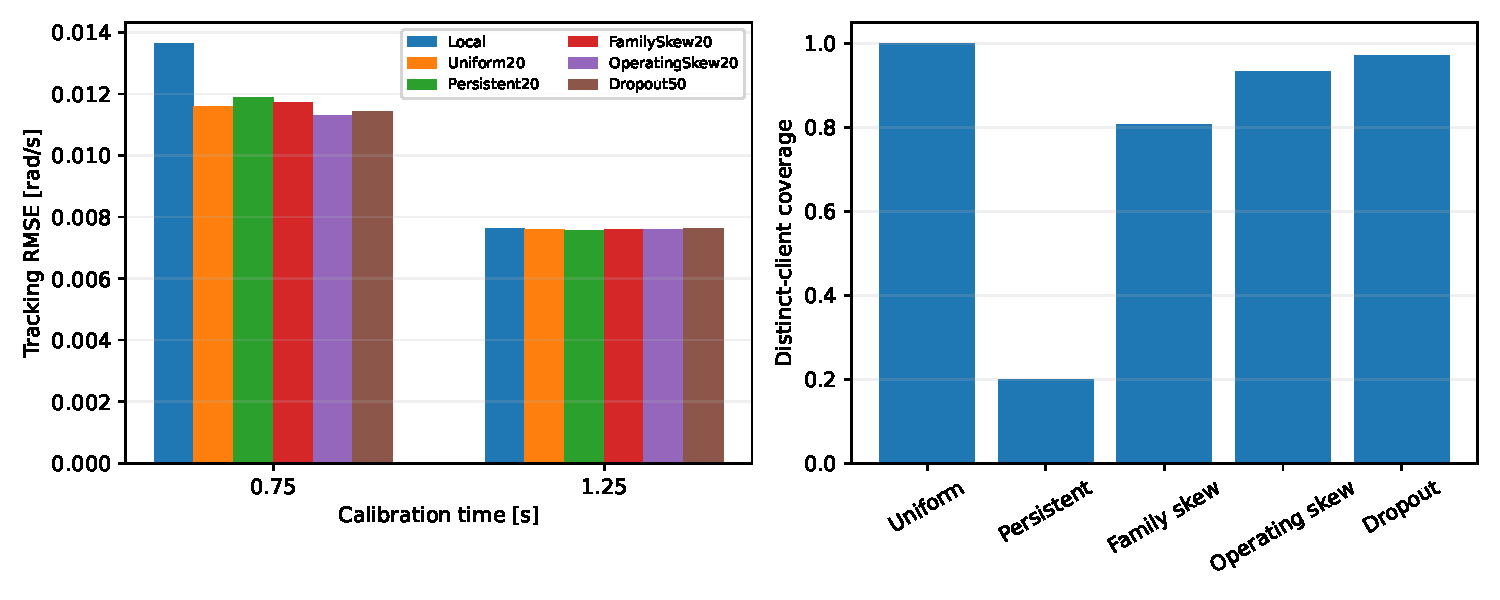
\includegraphics[width=0.93\linewidth]{../results/figures/experiment_9l_nonrandom_participation.pdf}
\caption{Aggregate tracking remains robust under all availability stresses,
but the persistent subset exposes a fleet-wise failure hidden by the mean.}
\label{fig:experiment9l}
\end{figure}

\paragraph{Aggregate result.}
Every predeclared aggregate gate passes. Persistent and family-skewed
participation degrade cold-start tracking from Uniform20 by only 2.70\% and
1.14\%; operating skew and matched dropout happen to improve the aggregate
mean. These improvements are not interpreted as benefits of biased or missing
updates: stochastic cohorts alter the selected group count and finite-sample
regularization. Their defensible interpretation is absence of aggregate harm.
All stressed methods retain a 12.83--17.17\% cold-start improvement over Local.
At 1.25~s every method is again within 0.8\% of Uniform20 and Local.

Dropout50 uses only 745 messages per fleet on average, versus 1296 for Uniform20,
yet covers 97.2\% of clients and preserves cold-start performance. Family and
operating skew also retain broad distinct-client coverage. Exact recovery of
the generating families is not required for useful control: Dropout50 has mean
ARI 0.588 while still improving Local in all ten fleets.

\paragraph{Persistent-subset failure.}
The aggregate result does not imply worst-case reliability. Persistent20 sees
only 20\% of clients, with mean minimum family and speed-category coverage of
15.5\% and 5.6\%. On seed 221 it selects a single group and becomes 34.43\%
worse than Local at 0.75~s. It nevertheless wins nine of ten fleets, so its
aggregate mean passes. This is a concrete failure mode: repeated participation
cannot compensate for missing population support.

The other stresses win every cold-start fleet comparison; their worst fleet
still improves Local by 5.47\% (family skew), 8.47\% (operating skew), and
9.00\% (dropout). Thus temporary message loss and strong but rotating bias are
substantially safer than a permanently narrow cohort.

\paragraph{Decision.}
Experiment 9L strengthens the partial-participation claim while defining its
boundary. The method tolerates reduced messages, dropout, and rotating
availability bias when cumulative population coverage remains broad. It is not
reliable when the same small subset participates indefinitely. A deployable
server should therefore monitor group/operating-region coverage and solicit
underrepresented clients or fall back to Local identification when support is
insufficient. This coverage-aware safeguard is a more direct next improvement
than increasing the number of communication rounds.

All 2400 fits converge and all 12600 nonlinear closed-loop evaluations remain
feasible. Seeds 226--235 remain reserved; 9L is a development robustness study,
not an additional blind confirmation.

\paragraph{Reproducibility.}
The protocol is in \path{code/config/experiment_9l.json}; the driver is
\path{code/experiments/experiment_9l_nonrandom_participation.py}. The reusable
cohort-controlled aggregation path is implemented in
\path{code/src/federated_lpv/federated_manifold.py}. Aggregate, seed-level,
coverage, gate, and provenance records are stored under \path{results/tables}.
